% Manifest-bound publication figure includes. Vector PDF is the publication path.

\begin{figure*}[t]
  \centering
  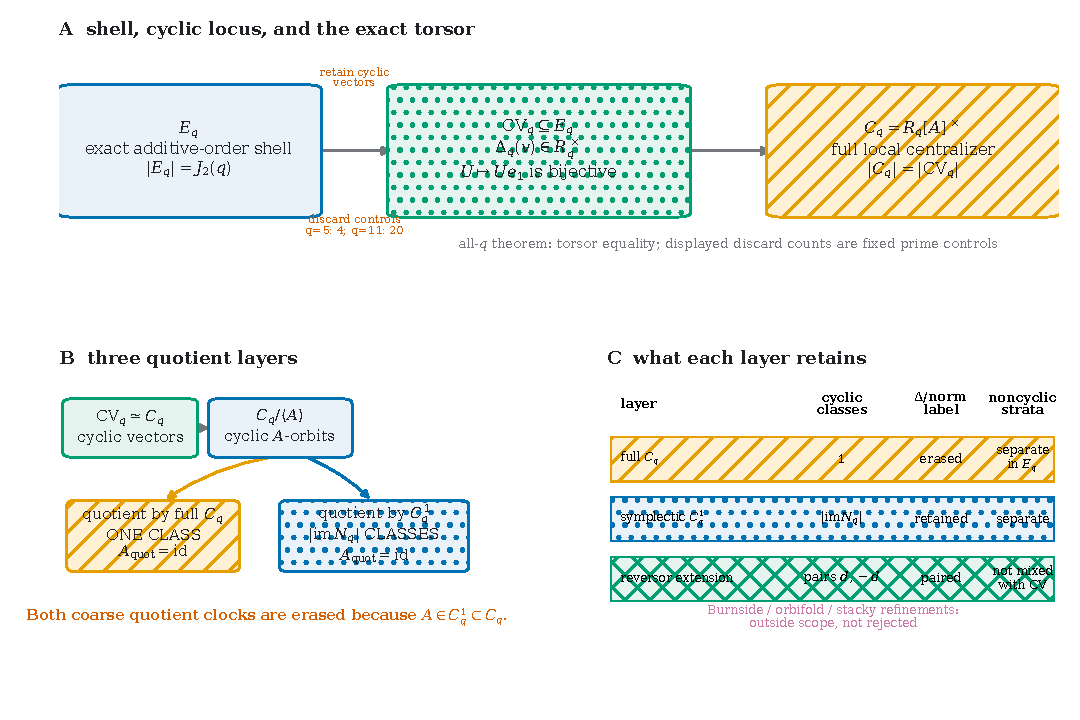
\includegraphics[width=\textwidth]{figures/fig1_quotient_layers.pdf}
  \caption{%
    Three quotient layers separate set compression from dynamical
    compression.  (A) The cyclic-vector locus
    $\mathrm{CV}_q\subseteq E_q$ is identified with the full local
    centralizer $C_q$ by $U\mapsto Ue_1$; split and ramified shells retain
    additional noncyclic strata.  (B) Cyclic $A$-orbits form
    $C_q/\langle A\rangle$.  The residual full-$C_q$ quotient has one class,
    while the determinant-one quotient has $|\operatorname{im}N_q|$ classes;
    both induced $A$ maps are the identity.  (C) The full, symplectic, and
    reversing layers retain different norm and noncyclic information.  The
    torsor and identity-map conclusions are proof-sourced for every $q$;
    shown discard counts are frozen prime controls.  Burnside, orbifold,
    stacky, groupoid, and twisted-sector refinements are outside scope, not
    ruled out.}
  \label{fig:quotient-layers}
\end{figure*}

\begin{figure*}[t]
  \centering
  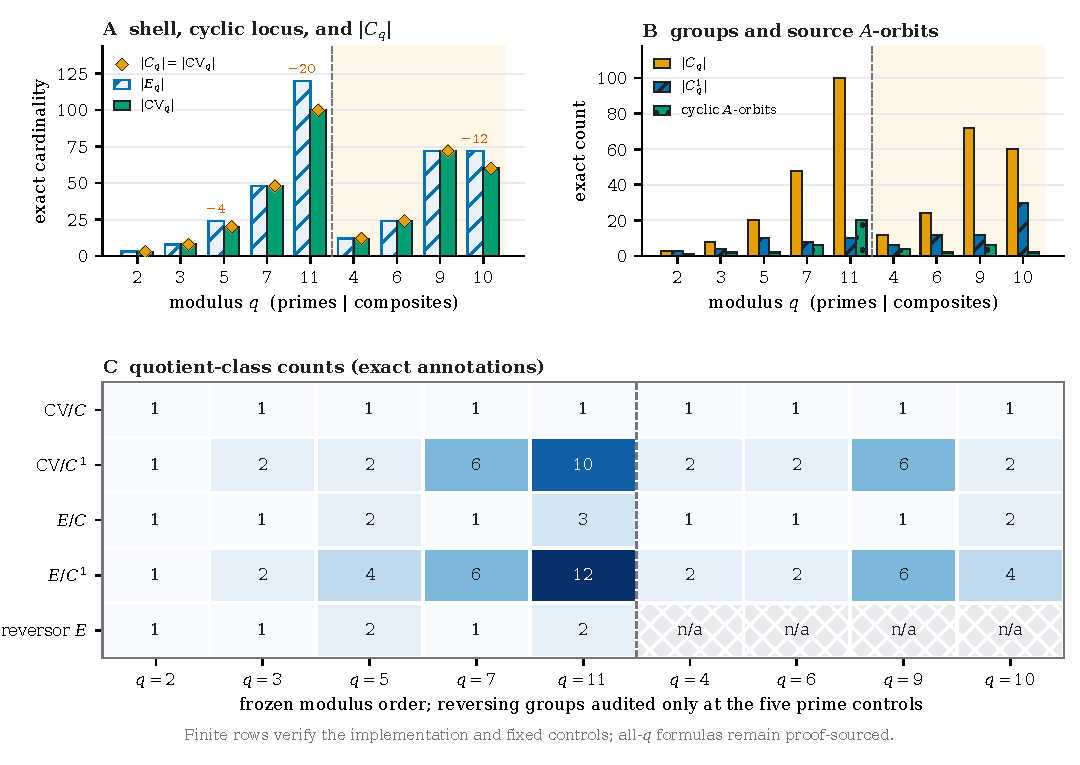
\includegraphics[width=\textwidth]{figures/fig2_nine_modulus_ledger.pdf}
  \caption{%
    Exact ledger for the frozen ordered moduli
    $q=2,3,5,7,11,4,6,9,10$.  (A) The cyclic locus can be smaller than the
    exact-order shell, but its cardinality always equals $|C_q|$ in the
    registered audit.  (B) Full-centralizer, symplectic-centralizer, and
    cyclic-$A$-orbit counts are kept distinct.  (C) The full cyclic quotient
    has one class at every control; the symplectic cyclic quotient has the
    exact norm-image count, and full-shell quotients expose the additional
    split/ramified strata.  Reversing groups were audited only at the five
    prime controls, so composite entries are marked not audited.  These
    development-seen finite rows verify the implementation and fixed
    controls; they do not prove the all-$q$ formulas.}
  \label{fig:nine-modulus-ledger}
\end{figure*}

\begin{figure*}[t]
  \centering
  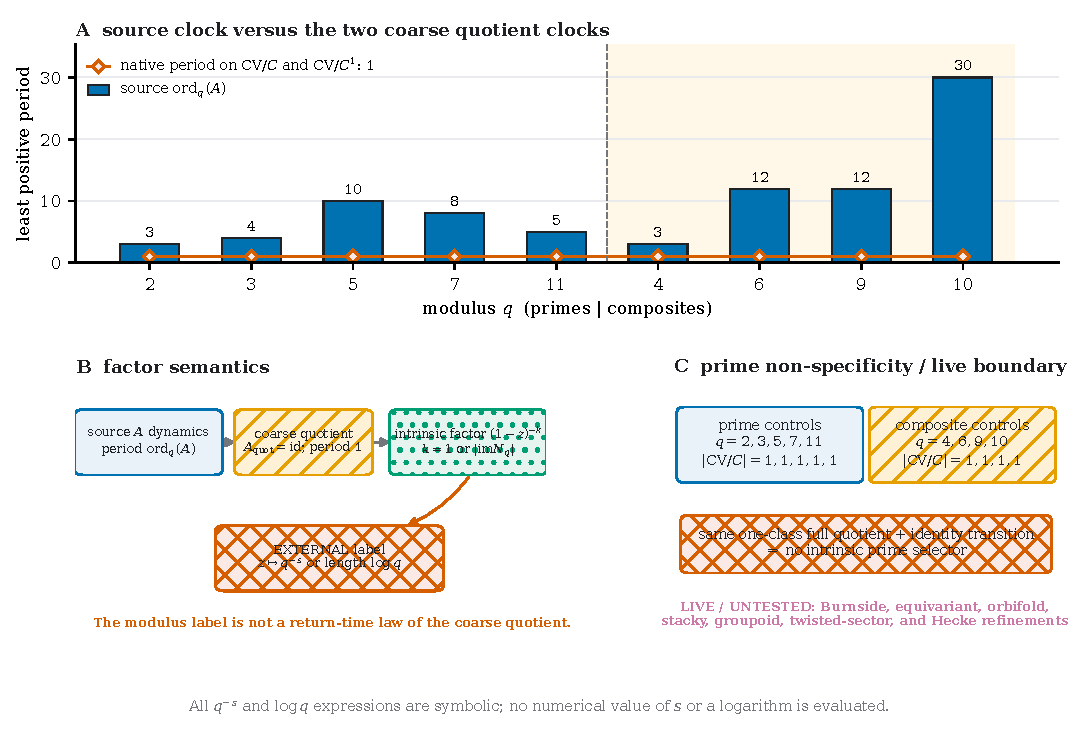
\includegraphics[width=\textwidth]{figures/fig3_clock_semantics.pdf}
  \caption{%
    Source periods do not survive either coarse centralizer quotient.  (A)
    The exact source period $\operatorname{ord}_q(A)$ varies across the nine
    controls, whereas both induced quotient maps have native primitive period
    one.  (B) The intrinsic identity-map factor is expressed in an abstract
    variable $z$; substituting $z=q^{-s}$ or assigning length $\log q$ is an
    external modulus specialization, not a quotient return-time law.  (C)
    every predeclared composite control has the same one-class full cyclic
    quotient as the primes, so the coarse mechanism supplies no intrinsic
    prime selector.  Enriched equivariant and Hecke constructions remain
    live but untested.  All $q^{-s}$ and $\log q$ expressions are symbolic;
    no numerical value is evaluated.}
  \label{fig:clock-semantics}
\end{figure*}

